% ======================================================================
\section{Forcing a positive zero mode}\label{sec:ordered}
% ======================================================================

\Cref{lem:spectral} bounds five local correlations $X_i$ from above in terms of the unknown zero mode $q$ and the nearest-neighbour correlation $g$. If we could also bound a suitable combination of the $X_i$ and $g$ from below by local information, we would obtain a lower bound on $q$. This section carries out this idea. The local information consists of exact identities and inequalities valid in every periodic box. Its combination is controlled through the law of the spins on a small shell.

\subsection{Geometry and the shell marginal}\label{sec:geometry}

Let
\[
 I=\{x\in\Z^3:\|x\|_1\le1\},\qquad \partial I=\{x:\|x\|_1=2\},
\]
regarded as subsets of $\T_L$ for $L\ge12$. The inner set $I$ has $7$ sites. The \emph{shell} $\partial I$ has $18$ sites: six \emph{axial} sites $\pm2e_i$ and twelve \emph{face} sites $\pm e_i\pm e_j$, $i<j$. There are no bonds within $\partial I$, since adjacent sites have $\ell^1$-norms of different parity. Every neighbour of $I$ lies in $I\cup\partial I$. The third shell $\{\|x\|_1=3\}$ consists of the eight \emph{corners} $\mathcal C=\{\pm1\}^3$, the six axial sites $\pm3e_i$, and the $24$ \emph{link sites} of type $(2,1,0)$, i.e.\ the images of $(2,1,0)$ under signed permutations. Each link site is adjacent to exactly one axial and one face site of $\partial I$. Each axial site lies on four links and each face site on two. Each corner is adjacent to three face sites. See \cref{fig:shells}.

\begin{figure}[t]
\centering
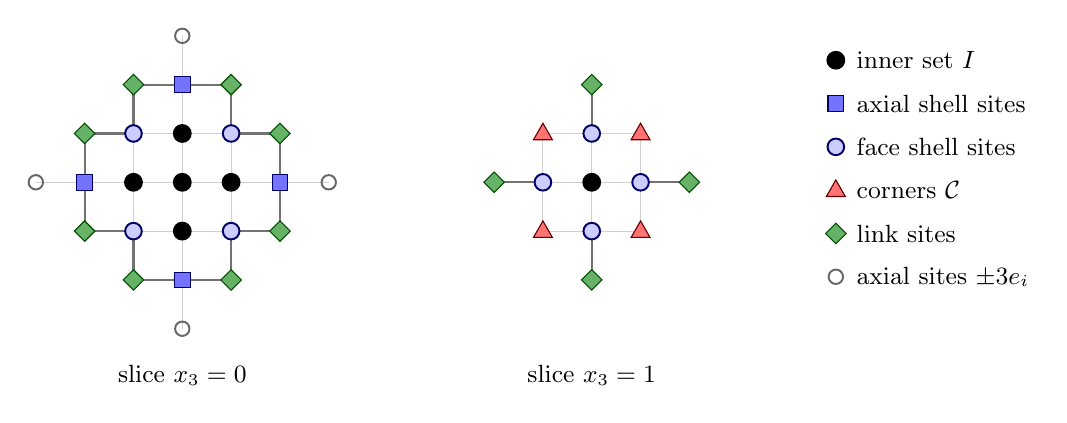
\begin{tikzpicture}[line cap=round]
\draw[black!18] (-1.860,0.000) -- (-1.240,0.000);
\draw[black!55,line width=0.8pt] (-1.240,-0.620) -- (-1.240,0.000);
\draw[black!55,line width=0.8pt] (-1.240,-0.620) -- (-0.620,-0.620);
\draw[black!55,line width=0.8pt] (-1.240,0.000) -- (-1.240,0.620);
\draw[black!18] (-1.240,0.000) -- (-0.620,0.000);
\draw[black!55,line width=0.8pt] (-1.240,0.620) -- (-0.620,0.620);
\draw[black!55,line width=0.8pt] (-0.620,-1.240) -- (-0.620,-0.620);
\draw[black!55,line width=0.8pt] (-0.620,-1.240) -- (0.000,-1.240);
\draw[black!18] (-0.620,-0.620) -- (-0.620,0.000);
\draw[black!18] (-0.620,-0.620) -- (0.000,-0.620);
\draw[black!18] (-0.620,0.000) -- (-0.620,0.620);
\draw[black!18] (-0.620,0.000) -- (0.000,0.000);
\draw[black!55,line width=0.8pt] (-0.620,0.620) -- (-0.620,1.240);
\draw[black!18] (-0.620,0.620) -- (0.000,0.620);
\draw[black!55,line width=0.8pt] (-0.620,1.240) -- (0.000,1.240);
\draw[black!18] (0.000,-1.860) -- (0.000,-1.240);
\draw[black!18] (0.000,-1.240) -- (0.000,-0.620);
\draw[black!55,line width=0.8pt] (0.000,-1.240) -- (0.620,-1.240);
\draw[black!18] (0.000,-0.620) -- (0.000,0.000);
\draw[black!18] (0.000,-0.620) -- (0.620,-0.620);
\draw[black!18] (0.000,0.000) -- (0.000,0.620);
\draw[black!18] (0.000,0.000) -- (0.620,0.000);
\draw[black!18] (0.000,0.620) -- (0.000,1.240);
\draw[black!18] (0.000,0.620) -- (0.620,0.620);
\draw[black!18] (0.000,1.240) -- (0.000,1.860);
\draw[black!55,line width=0.8pt] (0.000,1.240) -- (0.620,1.240);
\draw[black!55,line width=0.8pt] (0.620,-1.240) -- (0.620,-0.620);
\draw[black!18] (0.620,-0.620) -- (0.620,0.000);
\draw[black!55,line width=0.8pt] (0.620,-0.620) -- (1.240,-0.620);
\draw[black!18] (0.620,0.000) -- (0.620,0.620);
\draw[black!18] (0.620,0.000) -- (1.240,0.000);
\draw[black!55,line width=0.8pt] (0.620,0.620) -- (0.620,1.240);
\draw[black!55,line width=0.8pt] (0.620,0.620) -- (1.240,0.620);
\draw[black!55,line width=0.8pt] (1.240,-0.620) -- (1.240,0.000);
\draw[black!55,line width=0.8pt] (1.240,0.000) -- (1.240,0.620);
\draw[black!18] (1.240,0.000) -- (1.860,0.000);
\draw[black!60,line width=0.7pt] (-1.860,0.000) circle (2.6pt);
\filldraw[fill=green!50!black!60,draw=green!30!black] (-1.240,-0.620+0.13) -- (-1.240+0.13,-0.620) -- (-1.240,-0.620-0.13) -- (-1.240-0.13,-0.620) -- cycle;
\filldraw[fill=blue!55,draw=blue!40!black] (-1.240-0.10,0.000-0.10) rectangle (-1.240+0.10,0.000+0.10);
\filldraw[fill=green!50!black!60,draw=green!30!black] (-1.240,0.620+0.13) -- (-1.240+0.13,0.620) -- (-1.240,0.620-0.13) -- (-1.240-0.13,0.620) -- cycle;
\filldraw[fill=green!50!black!60,draw=green!30!black] (-0.620,-1.240+0.13) -- (-0.620+0.13,-1.240) -- (-0.620,-1.240-0.13) -- (-0.620-0.13,-1.240) -- cycle;
\filldraw[fill=blue!20,draw=blue!40!black,line width=0.7pt] (-0.620,-0.620) circle (3.0pt);
\fill[black] (-0.620,0.000) circle (3.4pt);
\filldraw[fill=blue!20,draw=blue!40!black,line width=0.7pt] (-0.620,0.620) circle (3.0pt);
\filldraw[fill=green!50!black!60,draw=green!30!black] (-0.620,1.240+0.13) -- (-0.620+0.13,1.240) -- (-0.620,1.240-0.13) -- (-0.620-0.13,1.240) -- cycle;
\draw[black!60,line width=0.7pt] (0.000,-1.860) circle (2.6pt);
\filldraw[fill=blue!55,draw=blue!40!black] (0.000-0.10,-1.240-0.10) rectangle (0.000+0.10,-1.240+0.10);
\fill[black] (0.000,-0.620) circle (3.4pt);
\fill[black] (0.000,0.000) circle (3.4pt);
\fill[black] (0.000,0.620) circle (3.4pt);
\filldraw[fill=blue!55,draw=blue!40!black] (0.000-0.10,1.240-0.10) rectangle (0.000+0.10,1.240+0.10);
\draw[black!60,line width=0.7pt] (0.000,1.860) circle (2.6pt);
\filldraw[fill=green!50!black!60,draw=green!30!black] (0.620,-1.240+0.13) -- (0.620+0.13,-1.240) -- (0.620,-1.240-0.13) -- (0.620-0.13,-1.240) -- cycle;
\filldraw[fill=blue!20,draw=blue!40!black,line width=0.7pt] (0.620,-0.620) circle (3.0pt);
\fill[black] (0.620,0.000) circle (3.4pt);
\filldraw[fill=blue!20,draw=blue!40!black,line width=0.7pt] (0.620,0.620) circle (3.0pt);
\filldraw[fill=green!50!black!60,draw=green!30!black] (0.620,1.240+0.13) -- (0.620+0.13,1.240) -- (0.620,1.240-0.13) -- (0.620-0.13,1.240) -- cycle;
\filldraw[fill=green!50!black!60,draw=green!30!black] (1.240,-0.620+0.13) -- (1.240+0.13,-0.620) -- (1.240,-0.620-0.13) -- (1.240-0.13,-0.620) -- cycle;
\filldraw[fill=blue!55,draw=blue!40!black] (1.240-0.10,0.000-0.10) rectangle (1.240+0.10,0.000+0.10);
\filldraw[fill=green!50!black!60,draw=green!30!black] (1.240,0.620+0.13) -- (1.240+0.13,0.620) -- (1.240,0.620-0.13) -- (1.240-0.13,0.620) -- cycle;
\draw[black!60,line width=0.7pt] (1.860,0.000) circle (2.6pt);
\node[font=\small] at (0.00,-2.45) {slice $x_3=0$};
\draw[black!55,line width=0.8pt] (3.960,0.000) -- (4.580,0.000);
\draw[black!18] (4.580,-0.620) -- (4.580,0.000);
\draw[black!18] (4.580,-0.620) -- (5.200,-0.620);
\draw[black!18] (4.580,0.000) -- (4.580,0.620);
\draw[black!18] (4.580,0.000) -- (5.200,0.000);
\draw[black!18] (4.580,0.620) -- (5.200,0.620);
\draw[black!55,line width=0.8pt] (5.200,-1.240) -- (5.200,-0.620);
\draw[black!18] (5.200,-0.620) -- (5.200,0.000);
\draw[black!18] (5.200,-0.620) -- (5.820,-0.620);
\draw[black!18] (5.200,0.000) -- (5.200,0.620);
\draw[black!18] (5.200,0.000) -- (5.820,0.000);
\draw[black!55,line width=0.8pt] (5.200,0.620) -- (5.200,1.240);
\draw[black!18] (5.200,0.620) -- (5.820,0.620);
\draw[black!18] (5.820,-0.620) -- (5.820,0.000);
\draw[black!18] (5.820,0.000) -- (5.820,0.620);
\draw[black!55,line width=0.8pt] (5.820,0.000) -- (6.440,0.000);
\filldraw[fill=green!50!black!60,draw=green!30!black] (3.960,0.000+0.13) -- (3.960+0.13,0.000) -- (3.960,0.000-0.13) -- (3.960-0.13,0.000) -- cycle;
\filldraw[fill=red!55,draw=red!40!black] (4.580,-0.620+0.13) -- (4.580-0.12,-0.620-0.08) -- (4.580+0.12,-0.620-0.08) -- cycle;
\filldraw[fill=blue!20,draw=blue!40!black,line width=0.7pt] (4.580,0.000) circle (3.0pt);
\filldraw[fill=red!55,draw=red!40!black] (4.580,0.620+0.13) -- (4.580-0.12,0.620-0.08) -- (4.580+0.12,0.620-0.08) -- cycle;
\filldraw[fill=green!50!black!60,draw=green!30!black] (5.200,-1.240+0.13) -- (5.200+0.13,-1.240) -- (5.200,-1.240-0.13) -- (5.200-0.13,-1.240) -- cycle;
\filldraw[fill=blue!20,draw=blue!40!black,line width=0.7pt] (5.200,-0.620) circle (3.0pt);
\fill[black] (5.200,0.000) circle (3.4pt);
\filldraw[fill=blue!20,draw=blue!40!black,line width=0.7pt] (5.200,0.620) circle (3.0pt);
\filldraw[fill=green!50!black!60,draw=green!30!black] (5.200,1.240+0.13) -- (5.200+0.13,1.240) -- (5.200,1.240-0.13) -- (5.200-0.13,1.240) -- cycle;
\filldraw[fill=red!55,draw=red!40!black] (5.820,-0.620+0.13) -- (5.820-0.12,-0.620-0.08) -- (5.820+0.12,-0.620-0.08) -- cycle;
\filldraw[fill=blue!20,draw=blue!40!black,line width=0.7pt] (5.820,0.000) circle (3.0pt);
\filldraw[fill=red!55,draw=red!40!black] (5.820,0.620+0.13) -- (5.820-0.12,0.620-0.08) -- (5.820+0.12,0.620-0.08) -- cycle;
\filldraw[fill=green!50!black!60,draw=green!30!black] (6.440,0.000+0.13) -- (6.440+0.13,0.000) -- (6.440,0.000-0.13) -- (6.440-0.13,0.000) -- cycle;
\node[font=\small] at (5.20,-2.45) {slice $x_3=1$};
\fill[black] (8.300,1.550) circle (3.4pt);
\node[right=4pt,font=\small] at (8.30,1.55) {inner set $I$};
\filldraw[fill=blue!55,draw=blue!40!black] (8.300-0.10,1.000-0.10) rectangle (8.300+0.10,1.000+0.10);
\node[right=4pt,font=\small] at (8.30,1.00) {axial shell sites};
\filldraw[fill=blue!20,draw=blue!40!black,line width=0.7pt] (8.300,0.450) circle (3.0pt);
\node[right=4pt,font=\small] at (8.30,0.45) {face shell sites};
\filldraw[fill=red!55,draw=red!40!black] (8.300,-0.100+0.13) -- (8.300-0.12,-0.100-0.08) -- (8.300+0.12,-0.100-0.08) -- cycle;
\node[right=4pt,font=\small] at (8.30,-0.10) {corners $\mathcal C$};
\filldraw[fill=green!50!black!60,draw=green!30!black] (8.300,-0.650+0.13) -- (8.300+0.13,-0.650) -- (8.300,-0.650-0.13) -- (8.300-0.13,-0.650) -- cycle;
\node[right=4pt,font=\small] at (8.30,-0.65) {link sites};
\draw[black!60,line width=0.7pt] (8.300,-1.200) circle (2.6pt);
\node[right=4pt,font=\small] at (8.30,-1.20) {axial sites $\pm3e_i$};
\end{tikzpicture}
\caption{Two horizontal slices of the neighbourhood of the origin used in \cref{sec:ordered}. The shell $\partial I=\{\|x\|_1=2\}$ separates the inner set $I$ from the exterior. Each link site of type $(2,1,0)$ joins one axial and one face shell site (dark bonds); summing over its spin couples the two shell spins and produces the factor $\xi^{d(b)}$ in~\eqref{eq:Psi}. The corners appear in the slices $x_3=\pm1$.}
\label{fig:shells}
\end{figure}


Let $b\in\{\pm1\}^{\partial I}$ denote a \emph{shell word} and let $\mu_L(b)$ be its marginal law under $\avg\cdot_L$. Write $H_I(\sigma_I,b)$ for the sum of $\sigma_x\sigma_y$ over the $36$ bonds with at least one endpoint in $I$, and put
\[
 Z_I(b)=\sum_{\sigma_I}e^{KH_I(\sigma_I,b)},\qquad
 f^I(b)=\frac1{Z_I(b)}\sum_{\sigma_I}f(\sigma_I,b)\,e^{KH_I(\sigma_I,b)}
\]
for functions $f$ of the spins in $I\cup\partial I$. By the Markov property, $\avg f_L=\mu_L(f^I):=\sum_b\mu_L(b)f^I(b)$. We call $f^I$ the \emph{conditional representative} of $f$. It is an explicit rational function of $r$ for each $b$. The group $\mathfrak G$ generated by the $48$ signed permutations of the axes and the global spin flip acts on shell words, and $\mu_L$ is $\mathfrak G$-invariant.

\subsection{Four families of rows}\label{sec:rows}

A \emph{row} is a function $\rho:\{\pm1\}^{\partial I}\to\R$ together with an inequality for $\mu_L(\rho)$ valid for all large even $L$. All rows below are averaged over $\mathfrak G$, so they are $\mathfrak G$-invariant. There are four families.

\begin{lemma}[Translation rows]\label{lem:translation}
Let $f$ be a function of the spins in a set $S$ and let $a\in\Z^3$ be such that $S$ and $S+a$ are contained in $I\cup\partial I$. Let $f_a$ denote the translate of $f$ to $S+a$. Then $\rT=f^I-f_a^I$ satisfies $\mu_L(\rT)=0$.
\end{lemma}

\begin{proof}
$\mu_L(\rT)=\avg f_L-\avg{f_a}_L=0$ by translation invariance of the periodic measure.
\end{proof}

The certificate uses $104$ translation rows $\rT_j$.

The second family comes from reflection positivity~\cite{FILS78,Bis09}. Let $\vartheta$ be the reflection of $\T_L$ in a pair of bond-bisecting planes orthogonal to a coordinate axis, as in the proof of \cref{lem:rotation}. Let $\T^\ell,\T^r$ be the two halves. Normalize each crossing bond weight as $e^{K\sigma\sigma'}=e^{-K}M_{\sigma\sigma'}$ with
\[
 M=\begin{pmatrix}r&1\\1&r\end{pmatrix}=M^{1/2}M^{1/2}.
\]
Inserting $M_{\sigma_x\sigma_{\vartheta x}}=\sum_{c=1,2}(M^{1/2})_{\sigma_xc}(M^{1/2})_{c\sigma_{\vartheta x}}$ on every crossing bond writes the torus weight as $\sum_{\mathbf c}\Xi_{\mathbf c}(\sigma^\ell)\Xi_{\mathbf c}(\vartheta\sigma^r)$, as in \cref{lem:rotation}. Consequently, for every collection of functions $F_{\mathbf c}$ of the spins of $\T^\ell$,
\begin{equation}\label{eq:RP}
 \sum_{\mathbf c}\Bigl\langle\!\Bigl\langle F_{\mathbf c}\,\vartheta F_{\mathbf c}\Bigr\rangle\!\Bigr\rangle\ge0,
\end{equation}
where $\langle\!\langle\cdot\rangle\!\rangle$ denotes the normalized sum with the split weights. The spin $\sigma_x$ at an endpoint of a crossing bond can be \emph{transported} to the auxiliary index. Since $\sigma_xM_{\sigma_x\sigma'}=(\mathrm{diag}(1,-1)M)_{\sigma_x\sigma'}$, replacing the column $M^{1/2}$ by $M^{-1/2}\mathrm{diag}(1,-1)M$ on the far side represents multiplication by $\sigma_x$. If both factors in~\eqref{eq:RP} carry a transported spin through the same crossing bond $\{x,\vartheta x\}$, the resulting Gram matrix is
\[
 (M^{-1/2}\mathrm{diag}(1,-1)M)^{\!\top}(M^{-1/2}\mathrm{diag}(1,-1)M)=\frac{M^3}{r^2-1}.
\]
Dividing it entrywise by $M$ gives the entries $c_0-\sigma_x\sigma_{\vartheta x}$, with the coefficient $c_0=u^{-1}+u$ of \cref{sec:infrared}. Thus every choice of coefficient vectors for finitely many local functions near the cutting plane, with or without transported spins, yields an inequality $\avg{\mathcal F}_L\ge0$ for an explicit local function $\mathcal F$.

\begin{lemma}[Reflection rows]\label{lem:reflection}
For each of the four coefficient vectors of \cref{cert:multipliers}, which have $112$ components, the conditional representative $\rA_k=\kappa_k\mathcal F_k^I$, normalized by a constant $\kappa_k>0$, satisfies $\mu_L(\rA_k)\ge0$.
\end{lemma}

The third family compares the region outside $I$ with a finite free graph. Let $\mathrm D$ be the graph obtained from $\T_L$ by deleting $I$ and all bonds incident to it. Let $\Gamma\subset\mathrm D$ be the free induced subgraph on the second and third shells and on the fourth-shell orbits of $(0,1,3)$ and $(0,2,2)$. It has $92$ sites and $150$ bonds. For $A\subset\partial I$ write $\chi_A(b)=\prod_{x\in A}b_x$.

\begin{lemma}[Deletion rows]\label{lem:deletion}
For $A,T\subset\partial I$ the function
\[
 \rD_{A,T}(b)=\frac{\chi_{A\triangle T}(b)-\avg{\chi_T}_\Gamma\,\chi_A(b)}{Z_I(b)}
\]
satisfies $\mu_L(\rD_{A,T})\ge0$.
\end{lemma}

\begin{proof}
Summing the torus weight over the spins outside $I\cup\partial I$ at fixed $b$ gives $\mu_L(b)=Z_I(b)Z_{\mathrm D}(b)/Z_L$, where $Z_{\mathrm D}(b)$ is the partition function of the Ising model on $\mathrm D$ with the shell spins fixed to $b$. Hence $F_A:=\sum_b\mu_L(b)\chi_A(b)/Z_I(b)$ is proportional, with a positive constant independent of $A$, to $\avg{\chi_A}_{\mathrm D}$. By \cref{lem:standard}(i) on $\mathrm D$, $\avg{\chi_{A\triangle T}}_{\mathrm D}=\avg{\chi_A\chi_T}_{\mathrm D}\ge\avg{\chi_A}_{\mathrm D}\avg{\chi_T}_{\mathrm D}$ and $\avg{\chi_T}_{\mathrm D}\ge\avg{\chi_T}_\Gamma$. With $\avg{\chi_A}_{\mathrm D}\ge0$ this gives $F_{A\triangle T}-\avg{\chi_T}_\Gamma F_A\ge0$, which is the claim.
\end{proof}

The certificate uses seven deletion rows $\rD_s$, each multiplied by $32\min_bZ_I(b)$ and symmetrized. The observable $\chi_{A\triangle T}(b)/Z_I(b)$ is integrated against the \emph{true} marginal $\mu_L$. No independence between $b$ and the interior is assumed.

The fourth family consists of the spectral rows of \cref{lem:spectral}. Let $g^I$ and $X_i^I$ be conditional representatives of local functions supported in $I\cup\partial I$ whose means are $g_L$ and $X_{i,L}$. Such representatives exist by translation invariance, since every displacement $x$ with $\|x\|_1\le4$ is realized by a pair of sites in $I\cup\partial I$. Put
\[
 \rS_i(b)=J_i^+\bigl(c_0-2g^I(b)\bigr)-X_i^I(b).
\]

\subsection{The residual}\label{sec:residual}

Write $y=\log r$, and let $a_j\in\mathbb Q$, $d_k,e_s,v_i\in\mathbb Q_{\ge0}$ be the multipliers of \cref{cert:multipliers}. The \emph{residual} and its zero-mode coefficient are
\begin{equation}\label{eq:residual}
 R_y(b)=-\sum_ja_j\rT_j(b)+\sum_kd_k\rA_k(b)+\sum_se_s\rD_s(b)+\sum_iv_i\rS_i(b),\qquad
 Q=\sum_iv_iP_i(\one).
\end{equation}

\begin{proposition}[Lower row inequality]\label{prop:lowerrow}
Let $L_k\to\infty$ be even integers along which $q_{L_k}$, $g_{L_k}$, the $X_{i,L_k}$ and $\mu_{L_k}(R_y)$ converge, and let $q=\lim q_{L_k}$. Then
\[
 0\le\lim_{k\to\infty}\mu_{L_k}(R_y)+Q\,q .
\]
\end{proposition}

\begin{proof}
By \cref{lem:translation,lem:reflection,lem:deletion}, $\mu_L(\rT_j)=0$, $\mu_L(\rA_k)\ge0$ and $\mu_L(\rD_s)\ge0$. By \cref{lem:spectral}, $\lim_k\mu_{L_k}(\rS_i)=J_i^+(c_0-2g)-X_i\ge-P_i(\one)q$. Multiply by the multipliers, of which all except the $a_j$ are nonnegative, and sum.
\end{proof}

\begin{certificate}[Rows and multipliers]\label{cert:multipliers}
The certificate consists of the $104+4+7+5=120$ rows as explicit local functions, specified by their supports, coefficient vectors and orbit data, and of their rational multipliers. The multipliers have the common denominator $10^6\cdot17887576666057000$. The translation multipliers $a_j$ have either sign, and all others are nonnegative. Moreover
\[
 Q=\frac{8943787728743670589}{8943788333028500000}.
\]
The residual $R_y$ is $\mathfrak G$-invariant. It is therefore constant on each of the $3236$ orbits of $\mathfrak G$ on $\{\pm1\}^{\partial I}$.
\end{certificate}

The values $R_y(b)$ have either sign, and $\max_bR_y(b)$ is positive. An upper bound for $\mu_L(R_y)$ that is strong enough to be combined with \cref{prop:lowerrow} must therefore use the structure of $\mu_L$. The rest of this section derives such a bound.

\subsection{A mixture representation of the shell marginal}\label{sec:mixture}

Put $\zeta=1/r=e^{-2K}$. With the normalization in which a bond contributes $1$ if its spins agree and $\zeta$ otherwise, we use the following constants:
\begin{equation}\label{eq:shellconstants}
 \xi=\frac{\zeta+\zeta^5}{\sqrt{(1+\zeta^6)(\zeta^2+\zeta^4)}},\qquad
 \eta=\frac{\zeta^2+\zeta^4}{1+\zeta^6},\qquad
 \rho_{\rm face}=\eta,\qquad \rho_{\rm axial}=\eta^2\phi_3,
\end{equation}
where $\phi_0=\zeta$ and $\phi_{m+1}=(\zeta+\zeta^4\phi_m)/(1+\zeta^5\phi_m)$. All of them lie in $(0,1)$ and are algebraic in $\zeta$. The quantities $\xi^2$, $\eta$, $\rho$ entering below are rational at rational $r$.

The basic device is elementary: if $0<\rho<1$ and $x=(x_+,x_-)$ is a positive vector with $\rho\le x_-/x_+\le\rho^{-1}$, then $x$ is a nonnegative combination of the two \emph{columns} $(1,\rho)$ and $(\rho,1)$. Applying it to a factor of the Gibbs weight introduces an auxiliary binary label, the choice of column, and summing over the label restores the weight.

\begin{lemma}[Mixture representation]\label{lem:mixture}
For $c\in\{\pm1\}^{\mathcal C}$, a \emph{corner source}, and $f\in\{\pm1\}^{\partial I}$, a \emph{field label}, define
\begin{equation}\label{eq:Psi}
 \Psi_{c,f}(b)=Z_I(b)\,\xi^{d(b)}\prod_{z\in\mathcal C}\bigl(\zeta^{k_z}+\zeta^{6-k_z}\bigr)\prod_{j\in\partial I}\rho_j^{\one\{b_j\ne f_j\}} .
\end{equation}
Here $d(b)$ is the number of links whose two shell endpoints disagree, which is even. The number $k_z$ counts the minus signs among the three face neighbours of $z$ and three copies of $c_z$. Finally $\rho_j=\rho_{\rm axial}$ or $\rho_{\rm face}$ according to the type of $j$. Let $\nu_{c,f}=\Psi_{c,f}/\sum_{b'}\Psi_{c,f}(b')$. Then for every even $L\ge12$ there are numbers $p_L(c,f)\ge0$ with $\sum_{c,f}p_L(c,f)=1$ such that
\begin{equation}\label{eq:mixture}
 \mu_L=\sum_{c,f}p_L(c,f)\,\nu_{c,f}.
\end{equation}
Moreover $p_L(gc,gf)=p_L(c,f)$ for $g\in\mathfrak G$.
\end{lemma}

\begin{proof}
Condition on the spins $\omega$ outside $I\cup\partial I\cup\mathcal C\cup\{\text{link sites}\}\cup\{\text{axial segments}\}$, where the axial segments are the sites $me_i$, $3\le|m|\le5$. Given $\omega$, the conditional weight of $b$ is $Z_I(b)$ times a product of factors, one for each corner, each link site and each axial segment. These are obtained by summing over the spin at that site or segment. We decompose each factor in turn.

\emph{Corners.} The three outward bonds of a corner $z$ contribute the vector $(\zeta^m,\zeta^{3-m})$ to the two values of $\sigma_z$, where $m$ is the number of minus signs among the outward neighbours. Its ratio lies in $[\zeta^3,\zeta^{-3}]$, so it is a nonnegative combination of $(1,\zeta^3)$ and $(\zeta^3,1)$. These columns are the weights produced by three outward neighbours of a common sign $c_z$. Summing over $\sigma_z$ then gives $\zeta^{k_z}+\zeta^{6-k_z}$.

\emph{Links.} A link site $t$ adjacent to the shell sites $i$ (axial) and $j$ (face) has four outward neighbours. If all four had the sign $a$, summing over $\sigma_t$ would give
\[
 (1+\zeta^6)\,\xi^{\one\{b_i\ne b_j\}}\,\eta^{(\one\{b_i\ne a\}+\one\{b_j\ne a\})/2},
\]
as one checks in the three cases $b_i=b_j=a$, $b_i=b_j=-a$ and $b_i\ne b_j$. For a general outward pattern the factor is a nonnegative mixture of the two cases $a=\pm1$. We call $a$ the \emph{preference} of the link.

\emph{Axial segments.} Tracing the three sites of an axial segment, each with four outward neighbours, gives a factor whose ratio in $b_i$ is bounded below by $\phi_3$. Combined with the $\eta^{1/2}$-factors of its four links, the total factor at an axial site has ratio in $[\rho_{\rm axial},\rho_{\rm axial}^{-1}]$. At a face site the two links give ratio in $[\eta,\eta^{-1}]$.

\emph{Field labels.} Decompose the total factor at each shell site $j$ into the columns $(1,\rho_j)$ and $(\rho_j,1)$, and call the chosen column $f_j$. Summing the products of all decomposition coefficients over $\omega$, against its true weight, yields nonnegative numbers $p_L(c,f)$ for which~\eqref{eq:mixture} holds after normalization. Symmetry follows from the $\mathfrak G$-invariance of $\avg\cdot_L$ and the covariance of each decomposition.
\end{proof}

The weights $p_L(c,f)$ depend on the exterior configuration. The labels at the two ends of a link are coupled through its preference, and the source labels are coupled through the exterior. The following two families of inequalities constrain them.

Fix a link $t$ joining the axial site $i$ and the face site $j$. For a field label $f$ write $f^{(i)}$ for $f$ with the bit at $i$ flipped.

\begin{lemma}[Bridge inequality]\label{lem:bridge}
If $f_i\ne f_j$, then for every $c$
\[
 p_L(c,f)\le\omega_i^{-1}p_L(c,f^{(i)})+\omega_j^{-1}p_L(c,f^{(j)}),\qquad
 \omega_k=\rho_k\,\frac{\rho_k/\eta-\rho_k}{1-\rho_k^2/\eta}>0 .
\]
\end{lemma}

\begin{proof}
Since $f_i\ne f_j$, one of the two labels disagrees with the preference $a$ of the link $t$, say $f_i\ne a$. Given $a$, the shell spins and the exterior, the local odds at $i$ in favour of $a$ are at least $\rho_i/\eta$. Expanding a vector with odds $x$ in the columns $(1,\rho_i)$ and $(\rho_i,1)$ gives coefficient odds $(x-\rho_i)/(1-\rho_ix)$. This is increasing in $x$, and is therefore at least $(\rho_i/\eta-\rho_i)/(1-\rho_i^2/\eta)$. For either value of $b_i$, the entries of the favourable and unfavourable columns have ratio at least $\rho_i$. Hence the unnormalized weight of $(c,f)$ on the event $\{a\ne f_i\}$ is at most $\omega_i^{-1}$ times the weight of $(c,f^{(i)})$ on the same event. Summing over the two values of $a$, with the roles of $i$ and $j$ exchanged on $\{a\ne f_j\}$, and then over the exterior gives the claim.
\end{proof}

For the corner sources, $\mathfrak G$ partitions $\{\pm1\}^{\mathcal C}$ into $14$ classes. Let $n_C$ be the size of the class $C$ and $p_C=\sum_{c\in C}\sum_fp_L(c,f)$ its mass. By symmetry each source in $C$ has mass $p_C/n_C$.

\begin{lemma}[Class odds]\label{lem:classodds}
Let $C,C'$ be classes such that a representative of $C'$ is obtained from one of $C$ by flipping a single corner source $c_z$. Let $m\in\{0,1,2,3\}$ be the number of the three corners adjacent to $z$ in the cube $\{\pm1\}^3$ whose source agrees with the new value of $c_z$. Then $p_{C'}/n_{C'}\ge\beta_m\,p_C/n_C$, where
\[
 \beta_m=\frac{\varpi-\zeta^3}{1-\zeta^3\varpi}\cdot\frac{\upsilon_m+\zeta^3}{1+\zeta^3\upsilon_m},\qquad
 \varpi=F(\zeta^4F(l^5))^3,\quad \upsilon_m=a_-^{3-m}a_+^m,
\]
with $F(x)=(\zeta+x)/(1+\zeta x)$, $l=F(\zeta^5)$ and $a_\pm=F(\zeta^4F(l^2\zeta^{\mp3}))$.
\end{lemma}

\begin{proof}[Sketch]
Fix the exterior and the other seven sources, and retain the corner $z$, its six axial two-step arms and the $21$ further neighbours of the arm endpoints. Each of the $21$ leaves has five neighbours outside. Tracing it through its arm gives an odds ratio of at least $l$. Tracing the three outer branches gives coefficient odds of at least $(\varpi-\zeta^3)/(1-\zeta^3\varpi)$ for the column associated with the new sign. Tracing the three inner branches and the corner spin, with $m$ matching sources, gives a further factor of at least $(\upsilon_m+\zeta^3)/(1+\zeta^3\upsilon_m)$. The comparison concerns unnormalized weights. It therefore survives the average over the exterior, including events of zero mass. Finally sum over field labels.
\end{proof}

\subsection{The upper cap}\label{sec:cap}

Write $\cR_{c,f}=\nu_{c,f}(R_y)$, so that $\mu_L(R_y)=\sum_{c,f}p_L(c,f)\cR_{c,f}$ by \cref{lem:mixture}. Each $\cR_{c,f}$ is a ratio of two explicit finite sums over $2^{18}$ shell words.

\begin{proposition}[Mixture cap]\label{prop:cap}
For each class $C$ with representative $c_C$, suppose given $\epsilon\ge0$, numbers $R^{\rm hi}_C\ge R^{\rm lo}_C$, a set $H_C\subset\{\pm1\}^{\partial I}$, and for each $f\in H_C$ a link $t(f)=\{i,j\}$ with $f_i\ne f_j$ and $f^{(i)},f^{(j)}\notin H_C$, such that
\[
 \cR_{c_C,f}\le R^{\rm hi}_C+\epsilon\ \ \text{for all }f,\qquad
 \cR_{c_C,f}\le R^{\rm lo}_C+\epsilon\ \ \text{for }f\notin H_C .
\]
Let $B_C$ be the largest total of the numbers $\omega_i^{-1}$, resp.\ $\omega_j^{-1}$, received by a single label outside $H_C$ under the assignment $f\mapsto f^{(i)},f^{(j)}$. Put $h_C=(B_CR^{\rm hi}_C+R^{\rm lo}_C)/(1+B_C)$. Finally let $\nu_{CC'}\ge0$ be multipliers indexed by the pairs of \cref{lem:classodds}, and
\begin{equation}\label{eq:Sclass}
 S_C=\frac1{n_C}\Bigl(\sum_{C'}\nu_{C'C}-\sum_{C'}\nu_{CC'}\beta_{CC'}\Bigr),\qquad
 \Uord=\epsilon+\max_C\bigl(h_C+S_C\bigr),
\end{equation}
where $\beta_{CC'}$ is the constant of \cref{lem:classodds} for the pair $(C,C')$. Then $\mu_L(R_y)\le\Uord$ for every even $L\ge12$.
\end{proposition}

\begin{proof}
Fix $C$ and write $p(f)=p_L(c_C,f)$. Summing \cref{lem:bridge} over $f\in H_C$ gives $p(H_C)\le B_C\,p(H_C^c)$. Since $R^{\rm hi}_C\ge R^{\rm lo}_C$,
\[
 \sum_fp(f)\cR_{c_C,f}\le p(H_C)R^{\rm hi}_C+p(H_C^c)R^{\rm lo}_C+\epsilon\,p(\cdot)
 \le\bigl(h_C+\epsilon\bigr)\,p(\cdot),
\]
because the middle expression is a weighted mean of $R^{\rm hi}_C$ and $R^{\rm lo}_C$ in which the weight of $R^{\rm hi}_C$ is at most $B_C/(1+B_C)$. The same bound holds for every source in $C$ by symmetry. Summing over classes, $\mu_L(R_y)\le\sum_Cp_C(h_C+\epsilon)$. By \cref{lem:classodds},
\[
 \sum_Cp_CS_C=\sum_{(C,C')}\nu_{CC'}\Bigl(\frac{p_{C'}}{n_{C'}}-\beta_{CC'}\frac{p_C}{n_C}\Bigr)\ge0 .
\]
Hence $\mu_L(R_y)\le\sum_Cp_C(h_C+S_C)+\epsilon\le\Uord$, since $\sum_Cp_C=1$.
\end{proof}

\subsection{The ordered certificate}

Let
\[
 r_b=\frac{3775}{2386},\qquad y_b=\log r_b,\qquad \Delta_b=\frac{4075}{10^{14}} .
\]

\begin{certificate}[Field caps at $r_b$]\label{cert:fields}
At $r=r_b$ the following data satisfy the hypotheses of \cref{prop:cap}.
\begin{enumerate}[label=\textup{(\alph*)}]
\item The values $R_{y_b}(o)$ on the $3236$ orbits are replaced by integer-grid approximations $\widetilde R(o)$. The common radius $\epsilon$ bounds $|R_{y_b}-\widetilde R|$, summed against the absolute values of the multipliers.
\item For each of the $14$ classes and each of the $2^{18}$ field labels, the ratio $\nu_{c_C,f}(\widetilde R)$ is compared with $R^{\rm hi}_C$, and for $f\notin H_C$ with $R^{\rm lo}_C$. This amounts to $14\cdot2^{18}=3\,670\,016$ comparisons with $R^{\rm hi}$ and $3\,661\,604$ comparisons with $R^{\rm lo}$. The sets $H_C$ contain $8412$ labels in total.
\item The six odds constants are bounded below on the grid $10^{-10}\Z$. The class odds $\beta_0,\dots,\beta_3$ have numerators $502492095$, $515270524$, $528601005$, $542501939$, and the flip weights $\omega_{\rm axial},\omega_{\rm face}$ have numerators $356890721$ and $5255754299$. These enter the $40$ directed one-flip comparisons between classes. The certificate also contains the assignment $f\mapsto t(f)$ on the $24$ links and $13$ nonzero class multipliers $\nu_{CC'}$.
\item The resulting number $\Uord(r_b)$ is negative, and
\[
 \Bigl\lfloor10^{15}L_b\Bigr\rfloor=215386342,\qquad L_b:=-\frac{\Uord(r_b)}{Q},
\]
with positive remainder.
\end{enumerate}
\end{certificate}

\begin{proposition}\label{prop:rb}
$m_+(\tfrac12y_b)^2\ge L_b>215386342\cdot10^{-15}$.
\end{proposition}

\begin{proof}
Choose a subsequence as in \cref{prop:lowerrow}, which is possible by compactness. By \cref{prop:lowerrow,prop:cap,cert:fields}, $0\le\Uord(r_b)+Qq$, i.e.\ $q\ge L_b$. Conclude with \cref{prop:order}.
\end{proof}

\subsection{Extension to an interval and the upper bound}

The proof of \cref{prop:rb} works at any $r$ for which the inequalities of \cref{cert:fields} remain valid. We keep all combinatorial data fixed: the rows, the multipliers, $J_i^+$, $Q$, the sets $H_C$, the assignment $t$, the class multipliers, and the frozen lower bounds for the six odds constants. We then bound the variation of the field ratios with $y=\log r$.

\begin{certificate}[Interval]\label{cert:interval}
On $r\in[r_b-\Delta_b,r_b]$ the following hold.
\begin{enumerate}[label=\textup{(\alph*)}]
\item Splitting $1/r\in[1/r_b,1/(r_b-\Delta_b)]$ into $16$ equal intervals and evaluating with outward rounding on the grid $2^{-120}\Z$, the six odds constants stay strictly above their frozen values. The least gap is at least $1171\cdot10^{-14}$.
\item The $y$-derivative of a single row is bounded by $144$, $228$, $57792$ and $14208$ for translation, spectral, reflection and deletion rows respectively. Summed against the absolute multipliers, this gives $|\partial_yR_y(b)|<8326$ for all $b$.
\item $|R_y(b)|<71/1000$ for all $b$ and $r$ in the interval.
\item $|\partial_y\log\Psi_{c,f}(b)|\le468$ for a suitable $b$-independent normalization of $\Psi_{c,f}$.
\item With $C_*=8326+468\cdot\frac{71}{1000}=\frac{2089807}{250}$, exact rational arithmetic gives
\[
 L_b-\frac{C_*\Delta_b}{Q(r_b-\Delta_b)}>\frac{84723}{10^{15}} .
\]
\end{enumerate}
\end{certificate}

The derivative constants in~(b) come from three facts. The $y$-derivative of the conditional representative of a $\pm1$-valued inner observable is at most $72$. One also has $0<J_i^+<1$ and $|\partial_yc_0|<12$. A normalized reflection row with $112$ components satisfies $\|v\|_1^2\le112\|v\|_2^2$. This gives $2\cdot72=144$, $3\cdot72+12=228$, $112(7\cdot72+12)=57792$ and $32(2\cdot72+300)=14208$, where $300$ bounds the derivative of the $150$-bond comparison correlations.

\begin{theorem}\label{thm:upper}
For every $r\in[r_b-\Delta_b,r_b]$, $m_+(\tfrac12\log r)^2>84723\cdot10^{-15}$. Consequently
\[
 e^{2K_c}\le r_b-\Delta_b<r_b-\frac{407}{10^{13}}=r_+ .
\]
\end{theorem}

\begin{proof}
Fix $r$ in the interval. By \cref{cert:interval}(a), \cref{lem:bridge,lem:classodds} hold with the frozen constants. For each $(c,f)$,
\[
 \partial_y\,\nu_{c,f}(R_y)=\nu_{c,f}(\partial_yR_y)+\mathrm{Cov}_{\nu_{c,f}}\bigl(R_y,\partial_y\log\Psi_{c,f}\bigr).
\]
By \cref{cert:interval}(b)--(d) and the Cauchy--Schwarz inequality, $|\partial_y\nu_{c,f}(R_y)|\le C_*$. Since $|y-y_b|=\log(r_b/r)\le(r_b-r)/r\le \Delta_b/(r_b-\Delta_b)$, every field ratio at $r$ exceeds its value at $r_b$ by at most $C_*\Delta_b/(r_b-\Delta_b)$. Raising both caps $R^{\rm hi}_C,R^{\rm lo}_C$ by this amount raises each $h_C$, and hence $\Uord$, by the same amount. \Cref{prop:cap} gives $\mu_L(R_y)\le\Uord(r_b)+C_*\Delta_b/(r_b-\Delta_b)$, and $Q$ does not depend on $r$. As in the proof of \cref{prop:rb}, $m_+^2\ge L_b-C_*\Delta_b/(Q(r_b-\Delta_b))$, which exceeds $84723\cdot10^{-15}$ by \cref{cert:interval}(e). The last assertion follows from \cref{cor:monotone}(ii) at $r=r_b-\Delta_b$ and from the identity $r_b-407\cdot10^{-13}=r_+$.
\end{proof}

\begin{remark}
The multipliers were optimized so that $\Uord(r_b)$ is negative at a point $r_b$ as far to the left as possible. The resulting lower bounds on $m_+^2$, about $2.2\cdot10^{-7}$ at $r_b$ and $8.5\cdot10^{-11}$ at $r_b-\Delta_b$, are accordingly small.
\end{remark}

\begin{proof}[Proof of \cref{thm:main}]
Combine \cref{thm:lower,thm:upper}. The decimal bounds in~\eqref{eq:main} and~\eqref{eq:mainK} are exact rational comparisons; see Appendix~\ref{app:arith}.
\end{proof}
